%\title{Overleaf Memo Template}
% Using the texMemo package by Rob Oakes
\documentclass[a4paper,11pt]{article}
\usepackage[english]{babel}
\usepackage{graphicx, lipsum}

% \usepackage{graphics} % for pdf, bitmapped graphics files
% \usepackage{epsfig} % for postscript graphics files
% \usepackage{amsmath} % assumes amsmath package installed
% \usepackage{amssymb}  % assumes amsmath package installed
% % \usepackage{multirow}
% \usepackage{url}
\usepackage{float}
%% Edit the header section here. To include your
%% own logo, upload a file via the files menu.
% \title{Problem Set 2 \\ \Large Advanced Methods in Applied Statistics}
% \author{Magnus Berg Sletfjerding}
% \date{\today}
\begin{document}
\begin{titlepage}
  \centering
  % \vfill
  \begin{figure}[H]
      % \vspace*{-2cm}
      \makebox[\linewidth]{
      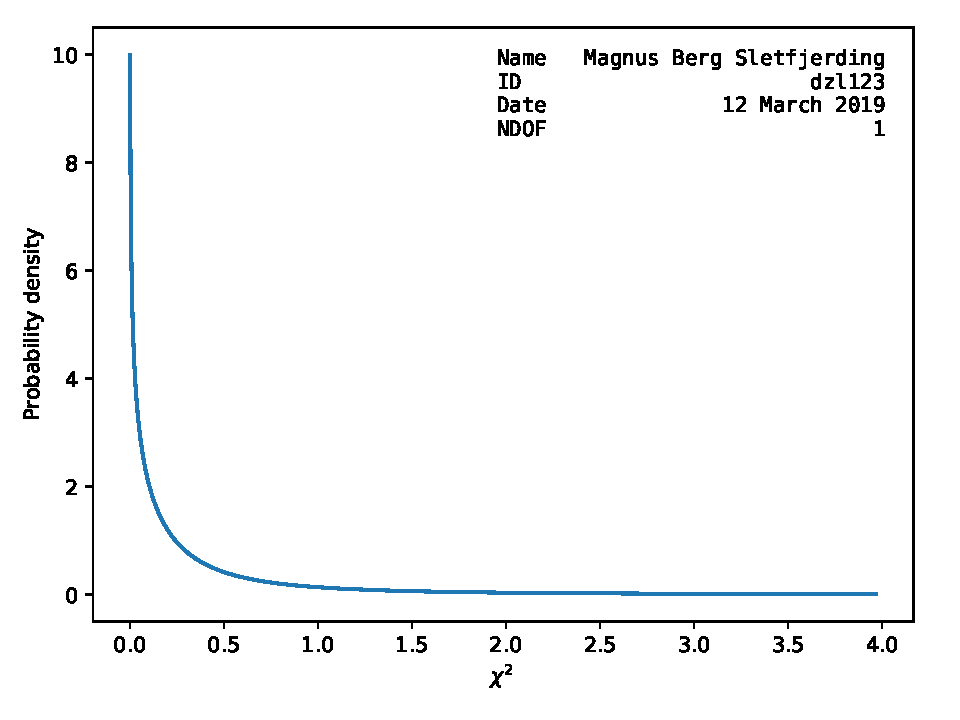
\includegraphics[width=1.5\linewidth]{../p1_chi2.pdf}
      }
      % \vfill
  \end{figure}
\end{titlepage}


\section{Problem 2 - Monte Carlo calculation of an arbitrarily drawn polygon}
I was amused by the shape of this polygon.
I generated points in the interval $x = (0,2), \; y = (0, 0.5)$ for the simple reason that its area is unity.
Using the \texttt{shapely} package, it was simple to check whether a point were inside the polygon or not.
I plotted the results, with the corresponding area in figure \ref{p2_bat}.
The area (0.166) also seems appropriate upon visual inspection.

\begin{figure}
  \makebox[\linewidth][c]{
  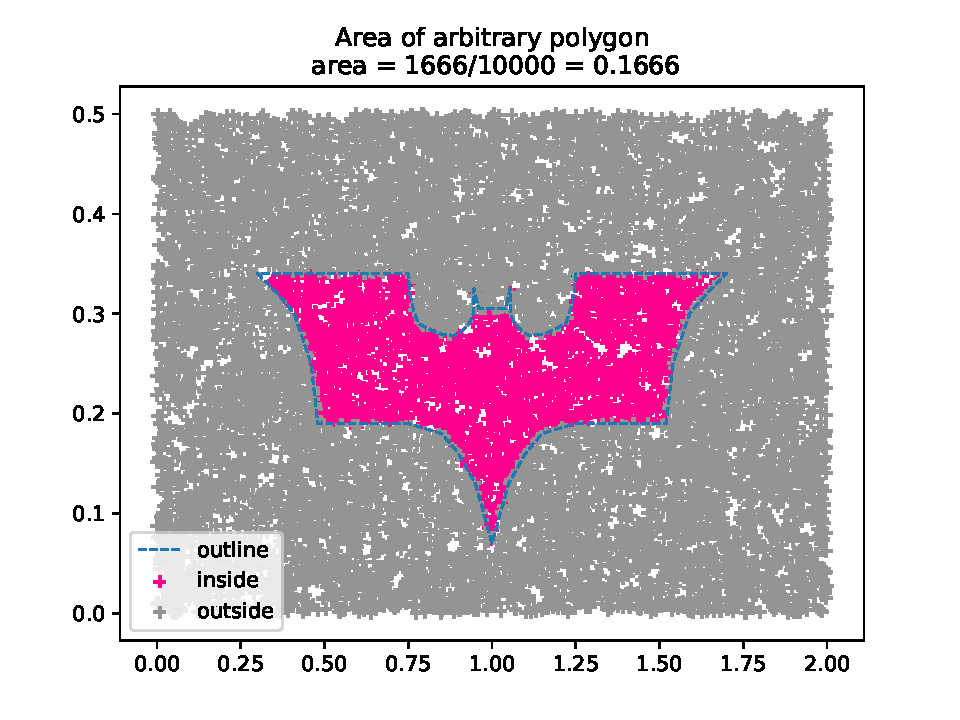
\includegraphics[width=\linewidth]{../p2_bat.pdf}
  }
  \caption{Problem 2}
  \label{p2_bat}
\end{figure}


\section{Problem 3 - Conditional probabilities for Slightly Evil Inc.}

This section was by far the most tricky to get right.
\subsection{Answers}
My answers are contained in the output from my code:
\begin{verbatim}
  Problem 3a:
Current aggregate defective rate: 0.03275
If defective, a PM is 18.32% likely to come from the facility A2
If defective, a PM is 23.66% likely to come from the facility A5
  Problem 3b:
  facility  defective  new_defective
0       A1      0.020       0.022143
1       A2      0.040       0.051667
2       A3      0.100       0.155000
3       A4      0.035       0.038750
4       A5      0.031       0.031000
  Problem 3c:
   facility  defective  new_defective
0        A1      0.020       0.022037
1        A2      0.040       0.059500
2        A3      0.100       0.119000
3        A4      0.035       0.074375
4        A5      0.022       0.023800
5        A6      0.092       0.180303
6        A7      0.120       0.313158
7        A8      0.070       0.070000
8        A9      0.110       0.180303
9       A10      0.020       0.297500
10      A11      0.070       0.396667
11      A12      0.060       0.270455
12      A13      0.099       0.396667
13      A14      0.082       0.743750
\end{verbatim}

\subsection{Explanation}
% TODO : explain the propagation of errors
\subsubsection{Problem 3a}
Finding the chance a defective pacemaker is from A2 facility calls for the use of Bayes' Theorem:

\[ P(A2 \vert D  ) = \frac{P(D\vert A2  ) * P(A2) }{P(D)} \]
Applying the already found values:

\[ P(A2 \vert D  ) = \frac{0.04 * 0.15 }{0.03275}  = 18.32 \%\]

Using the same formula, for all facilities, we find that:
\[ P(A5 \vert D  ) = \frac{0.031 * 0.25 }{0.03275}  = 23.66\%\]
Which is higher than all the others.
It makes intuitive sense, too, as the only other candidate, facility A4, still produces fewer defective devices than A5:
\[ P(A4 \vert D  ) = \frac{0.035 * 0.2 }{0.03275}  = 22.93\%\]

\subsubsection{Problem 3b and 3c}
Again, Bayes' Theorem shows itself handy.

In order to make all relative defective rates the same ($20\%$) we need to adjust all but one of the defective rates up.
(Analytically, it might make sense to increase the error rate for A5, as we know that it it the maximum.)

Doing so, I used the following formula to calculate the new defective rates from each factory:

\[
P(D \vert A_i)_{new, j} = \frac{P(A_j)}{P(A_i)}P(D\vert A_i)_{old}
\]
for all factories $A_i$, where $j$ indicates which factory's defective rate remains constant.

At this point, I only accepted the set of new defective rates where
\[
P(D \vert A_i)_{new} \geq P(D \vert A_i)_{old},   \forall   A_i
\]

Practically, this solution was scalable to be implemented on problem 3c as well.

\subparagraph{A realization that would have made the solution easier}

I realized after finishing this, that an alternative solution would be to start with the relative defecive rate ($1.0 / N$ where $N$ is the number of factories) and from there calculate the defective rates from there.
Nonwithstanding, I didn't implement this solution, as I believe that the original solution was sufficient (and scalable) enough to work for the whole problem.

\section{Problem 4 - Seawater}
\subsubsection{Problem 4a}
Numerical and graphical results are contained in figure \ref{p4_seawater}.


\begin{figure}[H]
  \centering
  \makebox[\textwidth][c]{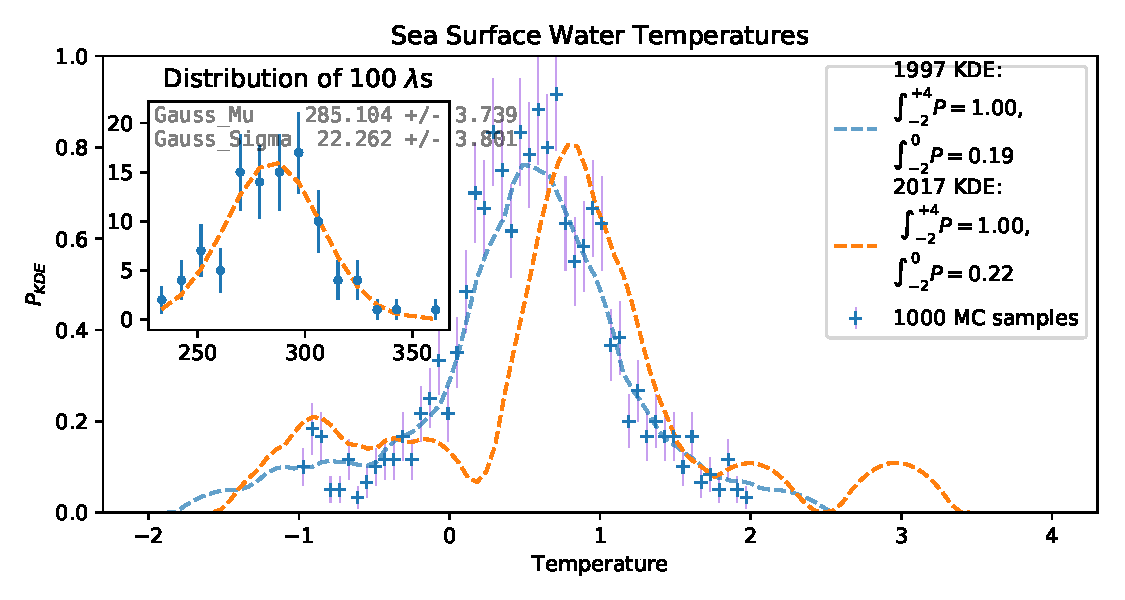
\includegraphics[width = 1.5\linewidth]{../p4_seawater}}
  \caption{Problem 4.
  After generating one lambda, I was surprised when the value was several orders of magnitude larger than 1.
  I therefore generated 100 lambdas and plotted the distribution, which seems to fit nicely with a gaussian.
The distribution of the values as a gaussian with mean 285 and sigma 22 demonstrates that the values of lambda can be estimated to fall in the interval $(241, 329)$ with 95\% confidence. }
  \label{p4_seawater}
\end{figure}

\section{Problem 5 - Particles}
\subsection{Problem 5a and 5b}

\begin{figure}[H]
  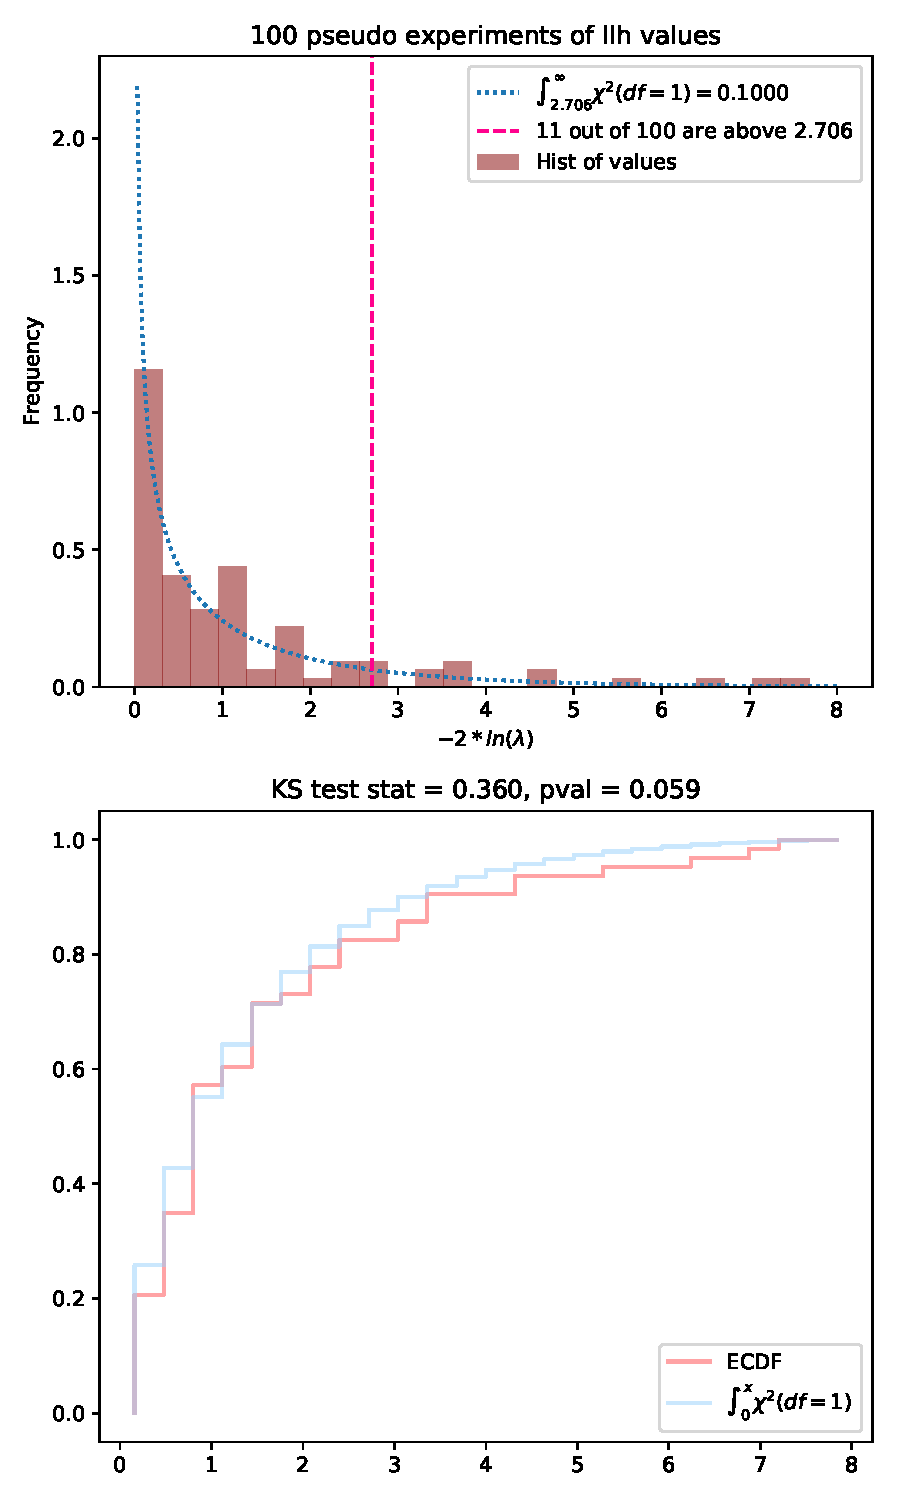
\includegraphics[width=\linewidth]{../p5_llhratios}
  \caption{Problem 5}
  \label{p5_llhratios}
\end{figure}

\subsection{problem 5c }
Using all 20000 events for a LLH test ...



\end{document}
